\documentclass[conference]{IEEEtran}
\IEEEoverridecommandlockouts

% Packages from the IEEE conference template, kept minimal for Milestone 2.
\usepackage{cite}
\usepackage{amsmath,amssymb,amsfonts}
\usepackage{graphicx}
\usepackage{textcomp}
\usepackage{xcolor}
\usepackage{booktabs}
\usepackage{array}
% --- added for the Deferrable Server double-hit timeline (Fig. 1) ---
\usepackage{tikz}
\usetikzlibrary{patterns}
% If you do NOT want the TikZ figure, delete the two lines above
% and the figure block in sections/milestone2.tex.
\usepackage[hidelinks]{hyperref}

\def\BibTeX{{\rm B\kern-.05em{\sc i\kern-.025em b}\kern-.08em
    T\kern-.1667em\lower.7ex\hbox{E}\kern-.125emX}}

\begin{document}

\title{Milestone 2: Scientific Contextualization and Tradeoff Analysis of the Deferrable Server}

\author{\IEEEauthorblockN{Md Rafiul Islam}
\IEEEauthorblockA{\textit{Electronic Engineering} \\
\textit{Hamm-Lippstadt University of Applied Sciences}\\
Germany \\
% Replace this line with your university email if required.
}}

\maketitle

\begin{abstract}
This milestone document contextualizes the Deferrable Server within real-time
scheduling. The focus is not polished final-paper prose, but structured
scientific reasoning: neighboring approaches, assumptions, the central
budget-preservation mechanism and its schedulability cost, engineering
tradeoffs, embedded-system consequences, and open questions for feedback.
\end{abstract}

\begin{IEEEkeywords}
Deferrable Server, real-time scheduling, aperiodic tasks, periodic tasks, embedded systems, schedulability, tradeoff analysis
\end{IEEEkeywords}

\section{Milestone 2: Scientific Contextualization and Tradeoff Analysis}

% ------------------------------------------------------------------
% Milestone style note: this is a structured technical briefing, not a
% finished paper. Reasoning is carried by bullets, tables, one formula,
% and one diagram, as recommended for M1-M3.
% ------------------------------------------------------------------

\subsection{Purpose and Scope}

This milestone places the Deferrable Server (DS) inside the broader landscape
of real-time scheduling and analyzes the tradeoffs it introduces, rather than
collecting loosely related papers.

\noindent\textbf{Core problem.} On a uniprocessor, serve unpredictable
\emph{aperiodic} requests with low response time \emph{without} causing the
co-scheduled \emph{periodic} hard real-time tasks to miss deadlines.

\noindent\textbf{Scope and model.}
\begin{itemize}
  \item Single preemptive processor; fixed-priority baseline (Rate/Deadline
        Monotonic \cite{liu1973scheduling}), with Earliest Deadline First (EDF)
        noted as the dynamic-priority counterpart.
  \item Periodic task $\tau_i$: known $(C_i, T_i, D_i)$ = WCET, period, deadline.
        Aperiodic job: unknown release time, soft or firm deadline.
  \item A \emph{server} is a schedulable entity with budget (capacity) $Q$ and
        period $P_s$ that reserves bandwidth $U_s = Q/P_s$ for aperiodic work.
\end{itemize}

\subsection{Design Space: Where the Deferrable Server Sits}

The mechanisms differ mainly in \emph{how reserved capacity is created,
preserved, or replenished}:
\begin{itemize}
  \item \textbf{Idle-time, no reservation:} Background Server.
  \item \textbf{Reserved budget, non-preserving:} Polling Server.
  \item \textbf{Reserved budget, budget-\emph{preserving} (fixed priority):}
        \underline{Deferrable Server}, Priority Exchange, Sporadic Server.
  \item \textbf{Slack-based (fixed priority):} Slack Stealing.
  \item \textbf{Bandwidth reservation under EDF (dynamic priority):}
        Total Bandwidth Server, Constant Bandwidth Server.
\end{itemize}
\noindent The DS is the \emph{simplest budget-preserving fixed-priority server}.
That niche --- better responsiveness than polling, far simpler than sporadic ---
is exactly what motivates studying it and its tradeoffs.

\subsection{Neighboring Approaches}

\begin{itemize}
  \item \textbf{Background Server:} aperiodic runs only when the CPU is idle.
        Zero interference on periodic tasks, but response time is poor and
        effectively unbounded under high periodic load.
  \item \textbf{Polling Server (PS):} full budget $Q$ at each period; if no
        request is pending at the polling instant, the budget is
        \emph{discarded}. Analyzable as an ordinary periodic task, but a
        request arriving just after a poll waits up to $P_s$.
  \item \textbf{Deferrable Server (DS):} full budget $Q$ at each period, but
        unused budget is \emph{preserved} until the period end. Improves
        aperiodic response; breaks the periodic-task equivalence (see
        Sec.~\ref{sec:doublehit}) \cite{lehoczky1987enhanced,strosnider1995deferrable}.
  \item \textbf{Priority Exchange (PE):} preserves budget by trading
        high-priority capacity for execution at lower priority levels when no
        aperiodic work is pending. Better utilization bound than DS, more
        bookkeeping, usually worse response than DS \cite{lehoczky1987enhanced}.
  \item \textbf{Sporadic Server (SS):} replenishes only the \emph{consumed}
        amount, one period after consumption starts. Avoids the double-hit, so
        it behaves like a periodic task and \emph{keeps the full
        Liu--Layland bound}; needs a replenishment queue
        \cite{sprunt1989aperiodic}.
  \item \textbf{Slack Stealing:} services aperiodic jobs at top priority using
        slack computed from the periodic schedule. Optimal aperiodic response
        under fixed priority, but high memory/compute cost
        \cite{lehoczky1992slack}.
  \item \textbf{Total Bandwidth Server (TBS, EDF):} assigns each job a deadline
        $d_k=\max(r_k,d_{k-1})+C_k/U_s$ and schedules under EDF. Cheap, high
        utilization \cite{spuri1996scheduling}.
  \item \textbf{Constant Bandwidth Server (CBS, EDF):} enforces a $(Q,T)$
        reservation by postponing the deadline on overrun, giving temporal
        isolation; basis of Linux \texttt{SCHED\_DEADLINE}
        \cite{abeni1998integrating}.
\end{itemize}

% ---------------- Table I: taxonomy / comparison ----------------
\begin{table*}[t]
\caption{Server-based mechanisms for aperiodic service. The Deferrable Server is the simplest budget-preserving fixed-priority option.}
\label{tab:server_comparison}
\centering
\renewcommand{\arraystretch}{1.25}
\begin{tabular}{p{2.3cm} p{4.0cm} p{3.2cm} p{2.6cm} p{2.3cm}}
\toprule
\textbf{Approach} & \textbf{Budget / replenishment} & \textbf{Schedulability basis} & \textbf{Aperiodic response} & \textbf{Cost / complexity} \\
\midrule
Background        & none; runs on idle CPU & no extra analysis & poor, unbounded & trivial \\
\midrule
Polling (PS)      & full $Q$ each $P_s$; discarded if idle at poll & equivalent periodic task & poor if request misses poll & low \\
\midrule
\textbf{Deferrable (DS)} & full $Q$ each $P_s$; \emph{preserved} within period & lowered RM bound (double-hit) & good & low \\
\midrule
Priority Exchange & high-prio budget exchanged to lower levels & better bound than DS & medium & medium \\
\midrule
Sporadic (SS)     & only consumed amount, one $P_s$ after use & full Liu--Layland bound & good & medium (replenish.\ queue) \\
\midrule
Slack Stealing    & none; uses computed slack & optimal (fixed prio.) & best & high (slack tables) \\
\midrule
TBS (EDF)         & deadline $d_k=\max(r_k,d_{k-1})+C_k/U_s$ & EDF, $U_{\text{tot}}\le 1$ & good & low--medium \\
\midrule
CBS (EDF)         & $(Q,T)$ reservation, deadline postponed & EDF, isolation & good & medium \\
\bottomrule
\end{tabular}
\end{table*}

\subsection{Central Mechanism and Its Cost: Budget Preservation and the Double-Hit}
\label{sec:doublehit}

\noindent\textbf{Mechanism.} Unlike the PS, the DS keeps unused budget within
its period instead of discarding it. This is the entire source of its improved
responsiveness.

\noindent\textbf{The cost (back-to-back / ``double-hit'').} Preserved budget can
be spent at the very \emph{end} of period $k$; the budget is then reset to a
full $Q$ at the \emph{start} of period $k{+}1$ and can be spent immediately.
The result is up to $2Q$ of \emph{contiguous} highest-priority execution in a
near-zero window (Fig.~\ref{fig:doublehit}). A periodic task with identical
$(Q,P_s)$ cannot produce this burst.

\noindent\textbf{Consequence for schedulability.} Because of the double-hit, a
DS \emph{cannot} be modeled as an equivalent periodic task, and the schedulable
periodic utilization drops. For a highest-priority DS with $P_s$ no larger than
all task periods, the least upper bound on schedulable periodic utilization is
\cite{lehoczky1987enhanced,strosnider1995deferrable}
\begin{equation}
  U_p^{\mathrm{lub}} \;=\; \ln\!\left(\frac{U_s + 2}{2U_s + 1}\right),
  \qquad U_s=\frac{Q}{P_s}.
  \label{eq:dsbound}
\end{equation}
\begin{itemize}
  \item $U_s \to 0 \Rightarrow U_p^{\mathrm{lub}} \to \ln 2 \approx 0.693$
        (the classic Liu--Layland bound is recovered).
  \item $U_s = 0.5 \Rightarrow U_p^{\mathrm{lub}} = \ln 1.25 \approx 0.223$:
        the periodic set is limited to $\sim$22\% utilization.
  \item Eq.~\eqref{eq:dsbound} is monotonically decreasing in $U_s$: more
        aperiodic bandwidth $\Rightarrow$ less guaranteed periodic bandwidth.
\end{itemize}
\noindent\textbf{Why SS is ``more controlled.''} The Sporadic Server schedules
its replenishment one period after consumption \emph{begins}, which
structurally prevents the $2Q$ burst. That is the precise technical reason SS
preserves the full Liu--Layland bound while DS does not
\cite{sprunt1989aperiodic}.

% ---------------- Fig 1: double-hit timeline ----------------
\begin{figure}[t]
\centering
\resizebox{\columnwidth}{!}{%
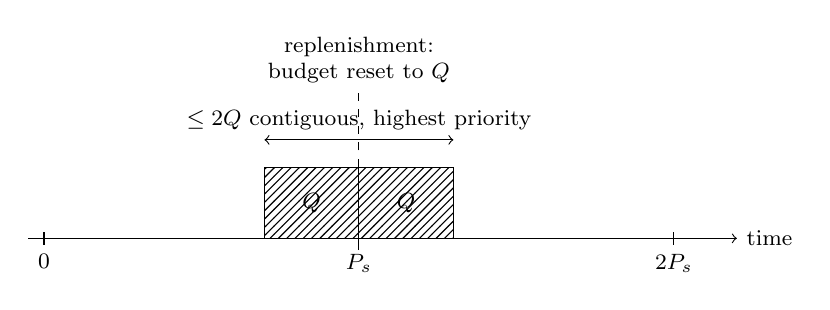
\begin{tikzpicture}[font=\footnotesize]
  % time axis
  \draw[->] (-0.2,0) -- (8.8,0) node[right]{time};
  \foreach \x/\lab in {0/0, 4/{$P_s$}, 8/{$2P_s$}}
      \draw (\x,0.08) -- (\x,-0.08) node[below]{\lab};
  % replenishment boundary
  \draw[dashed] (4,-0.15) -- (4,1.85);
  \node[anchor=south, align=center] at (4,1.85) {replenishment:\\budget reset to $Q$};
  % deferred budget at end of period 1: [2.8,4]
  \fill[pattern=north east lines] (2.8,0) rectangle (4,0.9);
  \draw (2.8,0) rectangle (4,0.9);
  % fresh budget at start of period 2: [4,5.2]
  \fill[pattern=north east lines] (4,0) rectangle (5.2,0.9);
  \draw (4,0) rectangle (5.2,0.9);
  \node at (3.4,0.45) {$Q$};
  \node at (4.6,0.45) {$Q$};
  % 2Q measurement
  \draw[<->] (2.8,1.25) -- (5.2,1.25);
  \node[anchor=south] at (4.0,1.25) {$\le 2Q$ contiguous, highest priority};
\end{tikzpicture}%
}
\caption{Deferrable Server ``double-hit'': unused budget pushed to the end of
one period, plus the full replenishment at the start of the next, yields up to
$2Q$ of contiguous highest-priority execution. A same-parameter periodic task
cannot generate this, which is why the DS lowers the schedulable periodic
utilization (Eq.~\eqref{eq:dsbound}).}
\label{fig:doublehit}
\end{figure}

\subsection{Assumptions (and Which Are Fragile in Practice)}

\begin{itemize}
  \item Single preemptive processor. \emph{[Fragile: multicore breaks the
        single-resource analysis.]}
  \item Server-management and context-switch overhead negligible.
        \emph{[Fragile on small MCUs.]}
  \item Periodic WCETs known and tight. \emph{[Fragile: WCET estimation is hard
        on cached/pipelined cores.]}
  \item Aperiodic demand bounded by the server; excess simply waits.
        \emph{[Firm/hard aperiodic deadlines are not guaranteed.]}
  \item Independent tasks, no shared resources / blocking.
        \emph{[Fragile: real systems need PIP/PCP for mutexes.]}
  \item Negligible release jitter; server period $\le$ task periods for
        Eq.~\eqref{eq:dsbound}. \emph{[Often only approximately true.]}
\end{itemize}

% ---------------- Table II: tradeoffs ----------------
\begin{table*}[t]
\caption{Engineering tradeoffs exposed by the Deferrable Server and its neighbours.}
\label{tab:tradeoffs}
\centering
\renewcommand{\arraystretch}{1.25}
\begin{tabular}{p{4.2cm} p{6.0cm} p{6.0cm}}
\toprule
\textbf{Tradeoff axis} & \textbf{What you gain (cheaper / simpler end)} & \textbf{What you pay (controlled / costly end)} \\
\midrule
Aperiodic response vs.\ periodic schedulability & DS preserves budget $\Rightarrow$ fast aperiodic service & lower guaranteed periodic utilization via Eq.~\eqref{eq:dsbound} \\
\midrule
Simplicity vs.\ no schedulability penalty & DS: trivial period-boundary replenishment & SS: replenishment bookkeeping, but full Liu--Layland bound \\
\midrule
Static vs.\ dynamic priority & RM + DS: simple, certifiable, widely supported & EDF + TBS/CBS: higher utilization, isolation, more complex runtime \\
\midrule
Offline guarantee vs.\ runtime flexibility & large $Q$: better aperiodic latency at runtime & large $Q$ raises $U_s$ and shrinks the periodic bound \\
\midrule
Memory/overhead vs.\ optimal response & DS: $O(1)$ state (counter + timer) & Slack Stealing: optimal response but slack tables / computation \\
\bottomrule
\end{tabular}
\end{table*}

\subsection{Consequences for Embedded and Real-Time Systems}

\begin{itemize}
  \item \textbf{Memory footprint.} DS needs only a budget counter and a period
        timer ($O(1)$); SS needs a bounded replenishment queue; Slack Stealing
        needs slack tables --- the heaviest.
  \item \textbf{Runtime overhead.} Roughly Background\,$<$\,Polling\,$\le$\,DS
        \,$<$\,SS\,$<$\,Slack Stealing. The scheduler's own WCET matters on
        constrained MCUs.
  \item \textbf{Predictability / certification.} Safety standards
        (e.g.\ DO-178C, ISO~26262) favour fully analyzable mechanisms; if DS is
        used, its worst-case $2Q$ interference must be explicitly budgeted.
  \item \textbf{RTOS mapping.} POSIX \texttt{SCHED\_SPORADIC} $\approx$ Sporadic
        Server; Linux \texttt{SCHED\_DEADLINE} $\approx$ CBS; the DS itself is
        rarely a native primitive and is usually \emph{emulated}.
  \item \textbf{Energy / event handling.} A budgeted server consolidates bursty
        aperiodic work into predictable windows, which is friendlier to
        DVFS/sleep policies than ad-hoc interrupt handling.
\end{itemize}
\noindent\textbf{Verdict.} The DS is a good fit when (a) the platform uses
fixed-priority scheduling, (b) soft aperiodic latency matters, and (c) $U_s$ is
small enough that the Eq.~\eqref{eq:dsbound} penalty is tolerable. It is a poor
\emph{sole} mechanism for hard or safety-critical aperiodic paths unless the
worst-case $2Q$ interference is fully accounted for; there SS or a reservation
(CBS) is usually preferable.

\subsection{Related-Work Status and Included vs.\ Excluded References}

\noindent\textbf{Status.} The narrow core (the Lehoczky--Sha--Strosnider server
family, synthesized by Buttazzo \cite{buttazzo2011hard}) is \emph{mature and
nearly closed}: the design space is well characterized. ``Sparse'' here means
few \emph{new primitives}, not few papers --- which is why this milestone
compares a fixed, well-defined set instead of accumulating weakly related work.

\noindent\textbf{Included (and why).}
\begin{itemize}
  \item DS papers \cite{lehoczky1987enhanced,strosnider1995deferrable} ---
        definitional; give the bound and the double-hit.
  \item Sporadic Server \cite{sprunt1989aperiodic} --- the direct ``fix'' to
        the DS schedulability penalty.
  \item Liu--Layland \cite{liu1973scheduling} --- the bound the DS is measured
        against.
  \item TBS / CBS / Slack Stealing
        \cite{spuri1996scheduling,abeni1998integrating,lehoczky1992slack} ---
        neighbouring families that bound the design space (EDF side, optimal
        response).
  \item Buttazzo \cite{buttazzo2011hard} --- unified analysis and notation.
\end{itemize}

\noindent\textbf{Excluded (and why).} General-purpose OS schedulers (e.g.\
Linux CFS), cloud/batch schedulers, global/partitioned multiprocessor
scheduling, and learning-based schedulers --- different assumptions and goals
(throughput/fairness, not hard deadlines on one CPU).

\subsection{Open Questions for Feedback}

\begin{itemize}
  \item For a concrete task set, is there a closed form for choosing $(Q,P_s)$
        that meets both Eq.~\eqref{eq:dsbound} and an aperiodic-latency target,
        or must it be found by search?
  \item Can the extra deadline-miss risk caused specifically by the DS's
        deferred budget (relative to a PS) be bounded per task?
  \item On a small MCU, when is the DS schedulability penalty cheaper than
        paying for SS replenishment bookkeeping?
  \item How does adding resource sharing (PIP/PCP blocking) interact with the
        server's budget accounting?
  \item Does the double-hit penalty change under deadline-monotonic scheduling
        with $D_i < T_i$?
\end{itemize}

% ---------------- Table III: checklist mapping ----------------
\begin{table}[t]
\caption{Mapping of M2 checklist items to this document.}
\label{tab:checklist}
\centering
\renewcommand{\arraystretch}{1.2}
\begin{tabular}{p{6.0cm} p{2.0cm}}
\toprule
\textbf{M2 checklist item} & \textbf{Addressed in} \\
\midrule
Compared approaches/assumptions (not just summarized) & Tab.~\ref{tab:server_comparison}, \ref{tab:tradeoffs} \\
$\ge 1$ neighbouring approach / paradigm & Neighboring Approaches \\
Related-work strength (strong/weak/sparse) and why & Related-Work Status \\
Scientific / engineering tradeoffs & Tab.~\ref{tab:tradeoffs}, Eq.~\eqref{eq:dsbound} \\
Embedded constraints (timing, memory, energy) & Consequences \\
Why selected references are relevant & Included references \\
Why excluded references are less relevant & Excluded references \\
\bottomrule
\end{tabular}
\end{table}

\begin{thebibliography}{00}

\bibitem{liu1973scheduling}
C.~L. Liu and J.~W. Layland, ``Scheduling algorithms for multiprogramming in a
hard-real-time environment,'' \emph{J. ACM}, vol.~20, no.~1, pp.~46--61, 1973.

\bibitem{lehoczky1987enhanced}
J.~P. Lehoczky, L.~Sha, and J.~K. Strosnider, ``Enhanced aperiodic
responsiveness in hard real-time environments,'' in \emph{Proc. IEEE Real-Time
Syst. Symp. (RTSS)}, 1987, pp.~261--270.

\bibitem{strosnider1995deferrable}
J.~K. Strosnider, J.~P. Lehoczky, and L.~Sha, ``The deferrable server algorithm
for enhanced aperiodic responsiveness in hard real-time environments,''
\emph{IEEE Trans. Comput.}, vol.~44, no.~1, pp.~73--91, 1995.

\bibitem{sprunt1989aperiodic}
B.~Sprunt, L.~Sha, and J.~P. Lehoczky, ``Aperiodic task scheduling for
hard-real-time systems,'' \emph{Real-Time Syst.}, vol.~1, no.~1, pp.~27--60,
1989.

\bibitem{lehoczky1992slack}
J.~P. Lehoczky and S.~Ramos-Thuel, ``An optimal algorithm for scheduling
soft-aperiodic tasks in fixed-priority preemptive systems,'' in \emph{Proc.
IEEE Real-Time Syst. Symp. (RTSS)}, 1992, pp.~110--123.

\bibitem{spuri1996scheduling}
M.~Spuri and G.~C. Buttazzo, ``Scheduling aperiodic tasks in dynamic priority
systems,'' \emph{Real-Time Syst.}, vol.~10, no.~2, pp.~179--210, 1996.

\bibitem{abeni1998integrating}
L.~Abeni and G.~Buttazzo, ``Integrating multimedia applications in hard
real-time systems,'' in \emph{Proc. IEEE Real-Time Syst. Symp. (RTSS)}, 1998,
pp.~4--13.

\bibitem{buttazzo2011hard}
G.~C. Buttazzo, \emph{Hard Real-Time Computing Systems: Predictable Scheduling
Algorithms and Applications}, 3rd~ed.\hskip 1em plus 0.5em minus 0.4em\relax
Springer, 2011.

\end{thebibliography}

\end{document}